%%%% PROCESAR con PdfLaTeX !!!!!


\documentclass[12pt]{book}
\usepackage{geometry}\geometry{top=2cm,bottom=2cm,left=2cm,right=2cm}
\usepackage{amssymb}
\usepackage{amsmath}
\usepackage{graphicx}
\usepackage{txfonts}
%\usepackage{hyperref}
\usepackage[hidelinks]{hyperref}
\usepackage[spanish]{babel}
\setcounter{tocdepth}{3}
\usepackage[usenames]{color}

\usepackage[hidelinks]{hyperref}
\hypersetup{
    colorlinks=true,
    linkcolor=black,
    filecolor=magenta,      
    urlcolor=cyan,
    pdftitle={Sharelatex Example},
    bookmarks=true,
%    pdfpagemode=FullScreen,
}


\begin{document}
\thispagestyle{empty}

\begin {center}

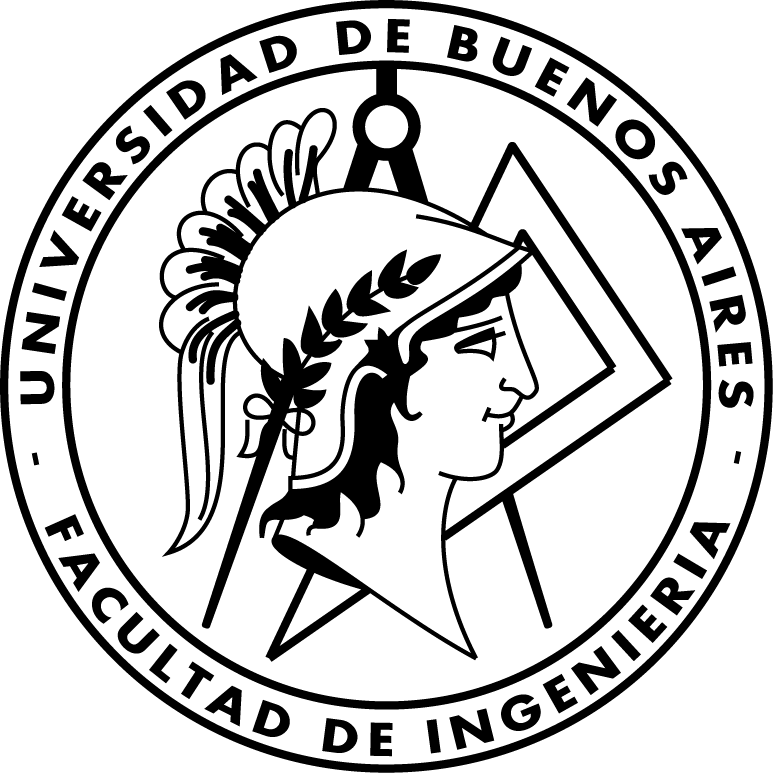
\includegraphics[scale=.4]{Logo-fiuba_big.png}

\medskip
UNIVERSIDAD DE BUENOS AIRES

Facultad de Ingenier\'ia

Departamento de Computación


\vspace{3cm}


\textbf{\large 75.17 Implantación de Sistemas} \\
\textbf{\large 76.56 Org. del Mantenimiento y la Implantación}

\vspace{2cm}


Este es un modesto aporte para los alumnos de la f\'acultad de ingenier\'ia  de la UBA de las carreras de licenciatura en an\'alsis de sistemas e ingenier\'ia inform\'atica.
De ninguna man\'era pretende ser una gu\'ia de estudio, ni remplaza las clases presenciales, el material oficial de la catedra esta disponible en el web site de la m\'ateria.
\\
\url{http://materias.fi.uba.ar/7510/}

\end {center}


\vspace{2.5cm}

\noindent Autor:\,	Isaac Edgar Camacho Ocampo
 
\noindent Carrera:\,	Licenciatura en An\'alisis de sistemas

\vspace{1cm}

\vspace{1cm}

\noindent Buenos Aires, 2019

\newpage


\tableofcontents
\chapter{CICLO DE VIDA, Modelo en cascada}
\section{ETAPAS}
\subsection{Elaboración}
\subsection{Implantación}
\subsection{Mantenimiento}

\chapter{LA IMPLANTACIÓN Y SUS ETAPAS}
\section{Método de Implantación y definición de la fecha de Puesta Operativa (go-live)}
\section{Calidad de la Información}
\section{Marco Normativo}
\section{Capacitación}
\section{Perfiles de Usuario}
\section{Pruebas de stress y de hardware y software}
\section{Plan de Corte}
\section{Plan de Contingencia}
\section{Análisis Post-Implantación}
\section{Ejercicios}


\subsubsection{Verdadero o falso}
	\begin{enumerate}
		\item \textbf{En el método de implantación en paralelo hay dos puestas operativas.}
				En Paralelo hay una sola PO. No se considera como PO el momento en que se implementa el 						nuevo sistema para su comparación con el actual.
		\item \textbf{Si hago una capacitación exhaustiva, hay mayor probabilidad de una implantación 							directa exitosa.} 
		
				El exito de la implementacion directa depende de La capacitación, las pruebas y la 								información, es decir necesitamos las tres, si solo tenemos capacitación no podremos 							garantizar el exito dela implantación.
		\item \textbf{Al no contar con la disponibilidad del usuario por falta de tiempo, entonces 								implementamos en forma directa.}
				
				La disponibilidad del usuario es necesaria para cualquier método de implantación que 							elijamos, de manéra que tendremos que determinar junto al responsable de la organización 
				como formaremos a los usuarios.
		\item \textbf{En el método de implantación escalonado hay varias puestas operativas con el mismo 						lapso de tiempo entre unas y otras.}
				En el método escalonado es cierto que hay varias PO, pero no siempre deben estar separados 
				un mismo lapso de tiempo.
	\end{enumerate}

\chapter{Calidad de la información}
\section{Objetivo:}
\section{Definición:}
\section{Situaciones que incitan a la migración de datos:}
\section{Proceso de migración/conversión/depuración:}
\section{Ejercicios}


\subsubsection{Verdadero o falso}
	\begin{enumerate}
		\item \textbf{Los criterios de depuración de datos deben ser definidos por la Gerencia “propietaria” 				de la información y aprobados por Auditoría.} Falso. \\
				Es verdadero que la gerencia dueña de la información debe definir los criterios de 								depuración, pero Auditoria hace un diagnostico de la empresa, para detectar riesgos, no 						aprueba criterios de depuración, simepre el que aprueba es el usuario.
				
		\item \textbf{La conversión de datos debe realizarse siempre justo antes de la puesta operativa dado
				que si se realiza antes los datos estarán desactualizados} 
				
				Es falso, porque todo depende de los datos ya sean dinámicos o estáticos, si son estaticos 						pueden convertirse en cualquier momento, no justo antes de la PO.
				
		\item \textbf{Si se desea realizar una carga automática de los datos estáticos se debe utilizar una
				interfase temporal}
				
				Los datos estáticos se van a transferir una sola vez, por lo tanto no va a ser permanente 
				el uso de esa interfaz, entonces es verdadera.
				
		\item \textbf{Durante la etapa de carga inicial del plan de implantación, podemos cargar los datos
				estáticos con las interfaces definitivas, y los datos dinámicos con las interfaces 								temporales.}
				
				Falso, porque es justo al revéz!!!.
	\end{enumerate}


\chapter{Manual de Usuario}Un manual de usuario, también llamado guía de usuario, es un documento de comunicación técnica destinado a dar asistencia a las personas que utilizan un sistema en particular.
\section{Objetivo:}
Crear un conjunto de descripciones y de instrucciones escritas que indicarán al usuario cómo
manejar y hacer funcionar el sistema.\\
Esta fase intenta crear la documentación para los usuarios.
\section{Definición:}
Se trata de una guía que ayuda a entender el funcionamiento de algo, por otro lado el usuario es aquiel que recibe la prestación de un servicio o es consumidor final de algún producto. El manual de usuario instruye al usuario en el uso del sistema y brinda la solución de problemas
que puedan ocurrir
\section{Elaborar el manual de usuario:}
Para elaborar un manual de usuario se debe tener en cuenta los siguientes puntos:
\begin{enumerate}
	\item Analizar a quien a dirigido:
	\item Coordinar el diseño del manual 	
\end{enumerate}

El manual de usuario debe contener:

{\setlength{\parindent}{64pt}
\begin{enumerate}
	\item \textbf{Índice}
	\item \textbf{Objetivo del sistema: para que fue creado dicho sistema}
	\item \textbf{Glosario}
	\item \textbf{Guía de uso:}

		\begin{enumerate}
			\item capturas de pantalla
			\item características claves del sistema
			\item entradas y salidas
			\item Interfases con otros sistemas			
			\item Especificaciones de mensajes de error 			
			
		\end{enumerate}

		
	\item \textbf{Sección de solución de problemas}
	\item \textbf{Mail, teléfono de soporte técnico}	
	\item \textbf{Preguntas frecuentes}
																															
\end{enumerate}

}%{\setlength{\parindent}{48pt}

\subsection{evitar los 13 pasos terribles}
\begin{enumerate}

	\item Evitar la facilidad de lectura
	\item Ocultar información crítica
	\item Utilizar juegos de caracteres indiscriminadamente
	\item Utilizar jerga indiscriminadamente
	\item Evitar lo evidente
	\item Intentar confundir
	\item Eliminar el uso de ejemplos
	\item Intentar desorganizar
	\item Incluir un índice inútil
	\item Guardar el manual en una carpeta poco manejable
	\item No comprobar el manual
	\item Tomar las sugerencias constructivas como un insulto personal 	
	\item No verificar la ortografía

\end{enumerate}


\section{Ejercicios}


\chapter{Capacitación de Usuario}
\parindent=8mm
Para la puesta en marcha de un nuevo sistema en una empresa, ya sea para mejorar uno anterior o para, optimizar una forma anterior de realizar los sucesos, hace falta capacitar al personal que va a utilizar dicho sistema

\section{Objetivo:}
\section{Determinar el personal a formar:}
\section{Determinar el alcance y la estrategia:}
\section{Capacitación y método de implantación}
Deberán considerarse cuestiones específicas del proyecto, como el método de implantación, en el Directo el sistema viejo y el nuevo no coexisten, por otro lado en el paralelo si coexisten pero el productivo es el sistema viejo, por lo tanto si hay problemas de capacitacion en el método paralelo tenemos chance de ir aprendiendo sobre la marcha, en tanto en el directo el impacto es mas prifundo porque si cargamos los datos mal, dedemos corregir errores.\\ \\
Si estamos en implantacion directa un indicadort importante es la asistencia a las capacitaciones por parte de los ususarios, ya que debemos asegurar un nivel minimo de usuarios capacitados para poder implantar, si no llegamos a un mínimo de gente entrenada entonces deberiamos postergar la fecha de PO, tambien deberiamos examinar a los usuarios.
		 \\
		 \\
		 
si es por étapas entonces la caacitación tambien va a ser por etapas.
\section{Ejercicios}


\subsubsection{Verdadero o falso}
	\begin{enumerate}
		\item \textbf{La capacitación de usuarios debe realizarse antes de la conversión de datos para 							depositar confianza en el control de la conciliación de los datos migrados.} 
		
		La capacitación es un proceso en que se hace en general con datos falsos, además los usuarios van a aprender a usar el sistema no a controlar la reconciliación de datos migrados, por lo tanto es falsa.
				
		\item \textbf{La capacitación a usuarios debe realizarse junto con la prueba del sistema a fin de 						que mientras los mismos aprenden detecten los errores del sistema.}
		
		Falso, porque al capacitar, eñ sistema ya debería haber sido probado, los errores durante la capacitación de usuarios es muy perjudicial porque genera desconfianza en los mismos.
				
	\end{enumerate}





\chapter{PLAN DE PRUEBAS}
Su objetivo consiste en confirmar que el sistema completo cumple los requisitos acordados del proyecto y es aceptado formalmente por la dirección correspondiente o el cliente.
\subsubsection{Para los desarrollos a medida:}
El entregable es el sistema funcionando, con lo cual las pruebas se realizan en la etapa correspondiente al
ciclo de vida.
\subsubsection{Para la implantación de una solución standard de mercado}
Las soluciones standard de mercado se tienen que configurar, realizar algunas adaptaciones, desarrollo de
interfaces con los sistemas con los que coexistirá.
Aun cuando la solución standard funciona, con la aplicación de configuraciones, adaptaciones se tienen
que probar.
En ambos casos, se deben realizar las pruebas de aceptación independientes.
\section{ESQUEMA TRADICIONAL DE PRUEBAS}
\section{PREPARAR Y REALIZAR LA PRUEBA DE FUNCIONAMIENTO}
\section{REALIZAR Y VERIFICAR LA PRUEBA DE ACEPTACIÓN}
\section{TIPOS DE PRUEBAS}
\section{EL SIGLO XXI Y LAS PRUEBAS}
\section{¿VERDADERO O FALSO?}

\begin{enumerate}
	\item \textbf{Las pruebas de aceptación del nuevo sistema deben ser realizadas por el personal de 						Sistemas del equipo de Implantación que conoce el comportamiento del mismo en detalle.}
	\item \textbf{No es necesario realizar pruebas de integración cuando se implanta un desarrollo a 						medida.}
	\item \textbf{Luego de la puesta operativa, no se pueden realizar más pruebas funcionales.}

\end{enumerate}


\chapter{MARCO NORMATIVO}El marco normativo, compuesto por políticas, manuales de autorización y de procedimiento, establece la posición de la 
compañía ante
la distribución de poder y las responsabilidades, determina quienes pueden
obligar económica y juridicamente a la empresa.

	\begin{enumerate}
		\item \textbf{Políticas:}
		\item \textbf{Manuales de Autorización:}
		\item \textbf{Manuales de Procedimientos:}
	\end{enumerate}

\section{Políticas}Las políticas se derivan de los objetivos generales de la compañía y son preceptos que sirven de guía para establecer
el curso de las acciones operacionales en la organización y para garantizar que los procesos y procedimientos. \\ \\
Las políticas orientan y proporcionan los límites y la dirección en la cual se desenvolverán las acciones generales que
luego a mayor nivel de detalle, se desarrollan en los manuales de autorización y de procedimientos.
laborales estén, consecuentemente, alineados con sus objetivos.\\ \\
Hay politicas de:
	\begin{enumerate}
		\item De Seguridad, salud y medio ambiente
		\item De Recursos humanos
		\item De Uso de recursos tecnológicos
	\end{enumerate}
\section{Manuales de Autorización}
Regula quienes toman las decisiones en la empresa, según puesto, monto u otros criterios. Lo altamente deseable
es que los manuales de autorización se encuentren embebidos dentro de los sistemas de aplicación, es decir que
según la transacción, el sistema determine el “vector de firmas” y rutee la transacción a las personas autorizadas
para evaluar y aprobar o rechazar la misma.
Según los principios de control interno, las decisiones relevantes deben ser tomadas como mínimo por 2 personas. \\
Ejemplos
	\begin{enumerate}
		\item		\textbf{De compras:} quien puede aprobar compras por determinados montos, condiciones, pagar anticipos y qué cosas se pueden comprar.
		\item		\textbf{De ventas:} quienes pueden aprobar ventas, condiciones, plazos de entrega, etc.
		\item		\textbf{De Producción:} quienes deciden que producir, para qué cliente, en qué línea de producción.
		\item		\textbf{De Recursos humanos:} quienes autorizan aumentos, promociones, pagos extraordinarios,
		incorporaciones, estructuras organizativas.
		\item		\textbf{De Administración y Finanzas:} quienes deciden las inversiones, condiciones de crédito, ajustes de
		inventario, etc.
	\end{enumerate}
\section{Manuales de Procedimientos}
Describen las operaciones que integran los procedimientos administrativos, en el orden secuencial de su ejecución,
y las normas que deben cumplir y ejecutar los miembros de la organización. Es un documento que les permite a los
empleados llevar a cabo sus labores de forma efectiva y con calidad desde el punto de vista de la gestión como de
control interno.
El procedimiento describe una serie de pasos claramente establecidos, que deben realizarse de la misma manera
independientemente de la persona que lo ejecute. Indica a las personas cómo realizar las tareas.\\ \\
Los componentes principales de cada procedimiento son:
\begin{enumerate}
	\item \textbf{la responsabilidad} - Quién realiza la acción
	\item \textbf{los pasos del procedimiento} - Qué acciones realizar, presentadas en un orden de tiempo lógico, y si existe
alguna dependencia de otros Procedimientos o Manuales de Autorización
		\item \textbf{los documentos suplementarios} - Qué cosas (pantallas, informes, formularios de entrada y registros de
operaciones de control) se relacionan con el paso del procedimiento y son necesarias para efectuarlo
\end{enumerate}

Ejemplos de manuales de procedimiento y contenidos generales:
\begin{enumerate}
	\item		\textbf{De compras de bienes y servicios:} quienes pueden gestionar las compras, quienes pueden comprar y qué,
		cuantas cotizaciones se requieren, modalidad de licitación (abierta, sobre cerrado, etc.),
	\itemº	\textbf{De compras menores:} modo de comprar artículos de bajo monto.
	\itemº	\textbf{De emisión de ofertas:} a qué precios
	\itemº	\textbf{De créditos:} a quienes se le otorgan créditos, con o sin garantía, plazos, refinanciaciones.
	\item	\textbf{De inventarios:} quienes son los responsables por su custodia, definir los puntos de repedido, a quienes se
		les puede entregar los bienes y bajo qué condiciones, cada cuanto se debe realizar el inventario y
		metodología.
\end{enumerate}

\section{Marco normatívo y su relación con el organigrama}
Un organigrama es la representación gráfica de la estructura de una empresa o cualquier otra organización, que incluye
las estructuras departamentales.\\
Los cargos que se mencionan en los Manuales de autorización y de procedimiento deben ser \textbf{consistentes} con los cargos
definidos en el organigrama.  \textbf{Las inconsistencias crean confusiones.}

\section{Ejercicio}
\begin{enumerate}
	\item \textbf{¿Todos los procesos requieren que estén procedimentados?} No!, sería imposible procedimentar todo proceso que se lleve adelante en una organización ya que esta, se compone de seres humanos, los procesos de negocio son los que obligatoriamente deben ser procedimentados por estar relacionados con los fines de la empresa y afectan a sus resultados.
	\item \textbf{En una compañía que no tiene normas ni procedimientos sino prácticas operativas informales
	conocidas por los empleados, ¿qué hay que desarrollar primero, el Manual de Autorizaciones o el
	Manual de Procedimientos?} El manual de procedimiento es lo primero que se debe implementar, ya que éste describe en forma clara los pasos que componen cada procedimiento, y si en algún paso se necesita la autorización de un superior vamos a poder definir tal permiso en el manual de autorizaciones, de lo contrario si realizamos primero el manual de autorizaciones no sabriamos qué ni a quién se debe autorizar.
\end{enumerate}
\textbf{Verdadero o falso}
\begin{enumerate}
	\item 	\textbf{El objetivo del manual de Normas y Procedimientos es establecer las tareas y responsabilidades 	que	tienen a su cargo los distintos sectores de una empresa.}
Falso!,
El marco normativo, compuesto por políticas, manuales de autorización y de procedimiento, establece la posición de la compañía ante determinados temas, la distribución de poder y las responsabilidades. Determina quienes pueden comprometer económica y financieramente a la empresa.		\\
De manéra que \textbf{establecer las tareas y responsabilidades 	que	tienen a su cargo los distintos sectores de una empresa} no es el única objetivo del mismo, ya que tambien degtermina quién puede obligar a la compañía, es decir tambien establece la jerarquía en la toma de desiciones.
	
	\item \textbf{El manual de procedimientos debe aprobarse durante la implantación en paralelo, antes de 				la 	puesta 	operativa del sistema de aplicación.}
	
	\item \textbf{Si en el nuevo sistema no existen normas y procedimientos aprobados formalmente, no es 			posible	determinar si existe concentración de funciones incompatibles en los distintos sistemas informáticos.}
	
	
	\item \textbf{	Siempre que se realicen cambios en los perfiles deben modificarse los manuales de normas 		y procedimientos relacionados con dichas funciones.}	
	
	
	\item \textbf{El manual de procedimientos define las responsabilidades de cada sector en cuanto a la 				operación 		del	sistema informático.}
	
	
\end{enumerate}



\chapter{PERFILES DE USUARIO}

Los perfiles de usuario dan permisos a los empleados sobre el sistema para que puedan ejecutar sus tareas. Los principios
de control interno que se deben seguir son:
\begin{enumerate}
	\item de los permisos mínimos necesarios, ni más ni menos
	\item segregados de funciones incompatibles
\end{enumerate}
La base para la construcción de los perfiles de usuario son los manuales de autorización y los manuales de procedimiento.
Los perfiles deben ser construidos en forma modular, de forma tal que se les asignen a las personas los módulos correspondientes a su puesto de trabajo.


\chapter{Repaso}
El modelo de ciclo de vida en cascada fue uno de los primeros modelos de desarrollo, -para sistemas de gran envergadura- no lo hacen recomendable ya que
hasta que todo está realizado, nada está terminado.
\\
Surgen entonces otras estrategias de ciclo de vida, Sus grandes grupos son Análisis, Diseño,
Elaboración, Implantación y Mantenimiento.\\

Hoy en dia tenemos agile, esto tiene pros y contras, para que una implementacion agile tenga exito es necesario que
\begin{itemize}
    \item debe haber una comunion entre el equipo de implantacion y los ususarios finales
    \item durante la etapa de construccion, los representantes de los usuarios debe tener peso.
    \item si ese alguien no conoce el negocio, no tiene poder de desicion, o no tiene representacion suficiente puede pasar que 
            cuando se presente el producto final, la alta dirección giga "esto no es lo que queriamos"
    \item LA FORTALEZA DEL REPRESENTANTE DE LA ORGANIZACIÓN
    \item EL CONOCIMIENTO DEL EQUIPO DE IMPLANTACIÓN DEL SISTEMA QUE SE VA A IMPLANTAR.
\end{itemize}

\section{Método de implantacion}
Hay dos criterios al momento de establecer el método de implantación.
\begin{itemize}
    \item En función de la coexistencia en el tiempo.
    \begin{itemize}
        \item Directo, deben existir todos los indicadores de control para que 
            \begin{itemize}
                \item que los usuarios esta capacitados \textbf{capacitacion}
                \item la informacion es buena \textbf{calidad de la información}
                \item que el sistema funciona de manera correcta. \textbf{pruebas}
            \end{itemize}
            si no tenemos estas variables bajo control, tenemos que considerar postergamos la fecha de PO, pero tambien postergaciones sucesivas
            de la PO, tiene impacto negativo.
        \item Paralelo, se analizan las diferencias ¿Qué pasa si hay diferencias?
                las diferencias se deben a 
                \begin{itemize}
                    \item \textbf{errores en el sistema viejo} puede ser que el sistema viejo haga algunos calculos mal, se deben avisar a la alta gerencia para que tome decisiones.
                    \item \textbf{errores en el sistema nuevo}
                    \item \textbf{hubo un cambio en las reglas de negocios}.
                \end{itemize}
        
    \end{itemize}
    \item En función de la modularidad.
    \begin{itemize}
        \item Bigbang.
        \item Escalonado por algún criterio.
    \end{itemize}
    Lo máx agresivo es directo y Big Bang, y lo maás conservador es escalonado por módulos.
\end{itemize}

\section{Fecha de PO}
Es el momento en que el nuevo sistema se pone productivo. O sea, está operativo y a partir del cual se
tomarán las decisiones con la información que proporcione, Hay que diferenciar entre PO y determinacion de la fecha de PO.
\\ \\
En proyectos grandes, para determinar la fecha de PO se deben tener en cuenta la experiencia, entender cuales son los desafios del proyecto, cuales sonlas situaciones complejas
para determinar una fecha de PO factible, casi siempre la empresa queire implantar lo antes posible, y van a presionar,
la determinar la fecha depende de el tamaño del proyecto y su conplejidad, la estructura organizativa, locaciones, si hay diferentes lenguajes
culturas etc., pero además la información  que necesitamos tambien puede estar desactualizada (proveedores etc) y obtener esos datos
talvez no dependa de nosotros entonces debemos tner es en cuenta para fijar la fecha de PO.





\chapter{Prácticas}
\section{Ejercicio 1}
Una empresa industrial con sede administrativa en Bs.As., planta en San Luis y sucursales en
Córdoba, Rosario, Mendoza y La Plata modificará su sistema de comunicaciones pasando de
transmisión telefónica a vía satélite, lo que posibilitará el replanteo de sus sistemas informáticos
discontinuando el método de actualización diferida de la información contable (batch),
adoptando el de actualización inmediata (on-line). Actualmente el procesamiento de la
información correspondiente a Ventas, Despacho, Facturación y Cobranzas está distribuido en
las distintas sucursales centralizando en Bs.As. la información contable (Contabilidad
Consolidada). Como el medio de comunicación utilizado es telefónico con tiempos de respuesta
inaceptables, diariamente (a la noche) cada sucursal envía un lote con toda la información
relacionada con ventas, facturación y cobranzas para que en Casa Central, a través de un proceso
batch se actualice la información en el Sistema Contable. De igual forma Casa Central transmite
un lote con toda la información actualizada de precios y stocks. A partir del nuevo método de
comunicación (listo en forma definitiva en 3 meses) se desea que cada vez que se realice una
operación (de venta, facturación, cobranza, etc.) se actualice inmediatamente la Contabilidad
de forma tal que los ajustes a la misma sean mínimos.
Desarrollar la fase de “Método de Implantación”, “Interfaces” y “Puesta Operativa”.
\subsection{Solucion} 
Hay una sede en buenos aires que es administrativa, 4 sucursales (que se comunican todos entre sí) y tenemos una planta de abastecimineto en San luis que se comunica con la sede administrativa y con las sucursales.
\\
Nos vamos aocupar de la sede central y las sucursales, no vamos a resolver la comunicacion entre la planta y las sucrusales porque implica medios de transporte.
\\
Hay que tener en cuenta algo muy importante, aqui el sistema productivo no cambia, sólo cambia el medio de comunicación, es decir las aplicaciones desde la funcionalidad no van a cambiar. \\ \\

\subsubsection{Método de Implantación}
Si no cambian las aplicaciones \textbf{NO PUEDO IMPLANTAR POR MÓDULO DENTRO DE LAS SUCURSALES}, si cambia solo la comunicación no hay cambio en el contenido, aqui el método de implantacion debe ser escalonado por sucursal y dentro de cada sucursal, directo big bang, ahora en la central tambien corresponde directo big bang pero debemos aclarar que vamos a tenes 2 metodos de comunicación (diferida y on-line) funcionado en paralelo, producto de que hay sucursales on-line y otras aún no implantadas batch, pero esto no implica un metodo paralelo porque no hay cambios en el sistema, no hay sistema viejo y nuevo.

\subsubsection{Puesta Operativa}
Vamos a tener cuatro puestas operativas una por cada sucursal y otra PO en casa central.

\subsubsection{Interfaces}
Supongamos que se implanta primero en la sucursal de Córdoba:
La nueva interfaz de Córdoba es ya la definitiva, es decir no va a cambiar.
Las otras tres sucursales (Rosario, La Plata y Neuquen) siguen manteniendo la misma forma de comunicación (batch) que, como van a ser reemplazadas, se consideran temporales porque vana a cambiarse.

Ahora implantamos Rosario,  entonces Cordoba y Rosario tiene interaces definitivas, el resto temporal
luego de la ultima PO (puesta operativa) todas son definitivas.

\subsubsection{Calidad de la Información}
Recordemos que solo cambia el momento de la comunicación, no hay cambio en la información, por lo tanto no hay carga inicial ni conversión ni migración y tampoco depuración, la uncica taréa que se puede hacer es la configuración de la central y las sucursales para los cambios por la transmision online, recordemos que la configuracion esta dentro de \textbf{Calidad de La información}


\chapter{Verdadero - Falso}
\begin{enumerate}
	\item	\textbf{La Auditoria es el área responsable de definir los controles internos en la compañía.}
	\item	\textbf{Cuando los procedimientos están desactualizados, es válido basarse para la definición de los perfiles de acceso en elsistema “nuevo”, los perfiles que están usando los usuarios en el sistema “viejo”}
	\item	\textbf{El dueño de los datos es el único responsable que aprueba los criterios para la depuración de la información}
\end{enumerate}


\chapter{Plan de Implantación - CheckList}
\section{Revisión de Hardware y Software}
\section{Método de Implantación}

\section{Puesta Operativa}
\section{Interfaces}
\section{Perfiles}
\section{Migración}
\section{Manual de Usuario}
\section{Manual de Normas y Procedimientos}
\section{Manual de Autorizaciones}
\section{Capacitación}
\section{Plan de Pruebas}
\section{Plan de Corte}
\section{Plan de Contingencia}
\section{Análisis Post-Implantación}


\chapter{AUDITORIA}
\section{¿Qué es una auditoría?}
Una auditoría es un proceso de verificación y/o validación del cumplimiento de una actividad según lo planeado y las directrices estipuladas.
\section{Riesgos:} Contingencia o proximidad de un daño. Combinación de la probabilidad de que se produzca un
evento y sus consecuencias negativas (R=Probabilidad x Impacto).
\section{Controles:} Acciones para mitigar la materialización (u ocurrencia) del riesgo.

\section{Riesgo Inherente}El riesgo inherente es propio del trabajo o proceso, que no puede ser eliminado del sistema; es decir, en
todo trabajo o proceso se encontrarán riesgos para las personas o para la ejecución de la actividad en sí
misma.
\section{Riesgo residual:} “Es aquel riesgo que subsiste, después de haber implementado controles.
\section{Riesgo de Control:} Se da cuando los controles implemenatados fallan.
\end{document}
